\documentclass{beamer}
\usepackage[spanish]{babel}
\usepackage[T1]{fontenc}
\usepackage[utf8]{inputenc}
\usepackage{lmodern}
\usepackage{amssymb}
\usepackage{graphicx}
\usepackage{amsthm}
\usepackage{amsmath}
\usepackage{mathtools}


\uselanguage{spanish}
\languagepath{spanish}


\def\tituloTesis{Métricas de mimetización acústico-prosódica en hablantes y su relación con rasgos sociales de diálogos}

\title{\tituloTesis}
\author{Juan Manuel Pérez}

\usetheme{Madrid}

\begin{document}

\beamertemplatenavigationsymbolsempty


\frame{\titlepage}



\begin{frame}
  \frametitle{¿Cómo dijo?}


\begin{itemize}[<+->]
  \item Sistemas de diálogo humano-computadora son cada vez más frecuentes, y sus aplicaciones comprenden una amplia gama de rubros
  \item Bien en la dimensión lingüística, mal en todo lo superestructural: emociones, actitudes, intenciones.
  \item Mimetización: Fenómeno insconsciente que se manifiesta a través de la adaptación de los hablantes. Fuertemente emparentada con el sentimiento de empatía.
  \item Objetivo del trabajo: Explorar y refinar una métrica de la mimetización acústico-prosódica, y validar que capture ciertas percepciones sociales en un corpus de diálogos en inglés.
\end{itemize}

\end{frame}



\section{Introducción}


Los sistemas de diálogo humano-computadora son cada vez más frecuentes, y sus aplicaciones comprenden una amplia gama de rubros: desde aplicaciones móviles, motores de búsqueda, juegos o tecnologías de asistencia para ancianos y discapacitados. Si bien es cierto que estos sistemas logran captar la dimensión lingüística de la comunicación humana, tienen un déficit importante a la hora de procesar y transmitir el aspecto superestructural de la comunicación oral, que radica en el intercambio de afecto, emociones, actitudes y otras intenciones de los participantes. Este problema puede verse en cualquier sistema que interactúe sintetizando lenguaje humano: por ejemplo, las aplicaciones telefónicas que atienden automáticamente a sus clientes \cite{pieraccini2005,raux2006}. Stanley Kubrick y Arthur C. Clarke predijeron esto a la perfección, cuando en ``2001: Una Odisea en el Espacio''(1968) dotaron a \emph{HAL} de una voz monótona y robótica, casi lobotomizada. Otro problema grave que sufren estos sistemas humano-computadora es que asumen que sus interacciones de ``a turnos'', cuando las conversaciones entre humanos suelen distar bastante de ese modelo.

Dentro de las cualidades del lenguaje oral, una de las más distintivas es la \emph{prosodia}, qué es la dimensión que capta \emph{cómo} se dicen las cosas, en contraposición a \emph{qué} se está manifestando. Posee varias componentes acústico-prosódicas: por ejemplo, el tono o pitch, la intensidad o volumen, la calidad de la voz, la velocidad del habla y otras. Un manejo adecuado de estas componentes es lo que, hoy día, distingue una voz humana de una artificial. Esta carencia de habilidad sobre la prosodia conlleva cierta dificultad en la interacción con agentes conversaciones, que suelen ser calificados como ``mecánicos'' o ``extraños'' en su forma de comunicarse. \cite{raux2006,ward2005}

En pos de mejorar el entendimiento entre agentes conversacionales y sus usuarios, resulta de vital importancia poder entender y modelar las variaciones prosódicas de la comunicación oral. Esto se traduciría tanto en una mejor apreciación de lo que quiere comunicar el usuario, como en una mayor naturalidad de la voz sintetizada por el agente.

\subsection{Mimetización}

En la literatura de Psicología del Comportamiento se ha observado con frecuencia que, bajo ciertas condiciones, cuando una persona mantiene una conversación, ésta modifica su manera de actuar aproximándola a la de su interlocutor. En una reseña de este tema se describe a este fenómeno como una ``imitación no consciente de posturas, maneras, expresiones faciales y otros comportamientos del compañero interaccional'' \cite[p. 893]{CHAR1999}  y conjeturan que es más fuerte en individuos con empatía disposicional. En otras palabras, personas con predisposición a buscar la aceptación social modifican su comportamiento en forma más marcada para aproximarlo a sus interlocutores

Esta modificación del comportamiento ha sido observada también en la manera de hablar. Por ejemplo, los interlocutores adoptan las mismas formas léxicas para referirse a las cosas, negociando tácitamente descripciones compartidas, en especial para cosas que resulten poco familiares \cite{BRE1996}. Estudios más recientes sugieren que esto también es cierto para el uso de estructuras sintácticas \cite{REI2006}. Este fenómeno subconsciente es conocido como mimetización, alineamiento, adaptación o convergencia y también con el término inglés \entrainment. Se ha mostrado que juega un rol importante en la coordinación de diálogos, facilitando tanto la producción como la comprensión del habla en los seres humanos\cite{nenkova2008,gravano2015backward}. En nuestro caso, nos interesa principalmente el \entrainment de la prosodia.

\subsection{Midiendo la mimetización}

Muchos estudios han examinado la mimetización prosódica, listados en \cite{DEL2013}. Un número importante de ellos se han basado en la premisa de la mimetización como un fenómeno lineal, en el cual la convergencia ``va sucediendo'' a lo largo de la conversación \cite{burgoon1995interpersonal}. Estos estudios dividen las conversaciones en varias partes, y verifican que la diferencia absoluta entre los valores medios (de las variables \ap) y sus desviaciones se aproxime en las últimas partes de la interacción. Sin embargo, este enfoque de la mimetización niega su faceta dinámica: los interlocutores pueden estar inactivos y luego hablar, pueden pasar por varias etapas como escuchar, pensar, discutir un punto, etc. En \cite{levitan2011measuring} se reportó que éste es un fenómeno no sólamente lineal, sino también dinámico, donde los interlocutores van coincidiendo en el análisis por turnos.

Un problema común que surge a la hora de calcular estas métricas es el hecho de que las conversaciones no están alineadas en el tiempo, ni se dan en turnos de duración constante. Nos preguntamos entonces qué partes del diálogo de un hablante deberían compararse con qué otras partes de su par. Un enfoque de comparar interlocuciones uno a uno es demasiado simple y no captura situaciones de diálogo reales, mucho más dinámicas y con solapamiento casi constante.

Para atacar estos inconvenientes, utilizamos el método \TAMA(Time Aligned Moving Average) \cite{KOU2008}, que consiste en separar en ventanas de tiempo el diálogo, y promediar los valores de las variables prosódicas dentro de cada una. Este método es muy similar a aplicar un filtro de Promedio Móvil (Moving Average), lo que da el nombre a la técnica. Al separar el diálogo en ventanas de tiempo, podemos construir dos series de tiempo en base a cada interlocutor. Estas abstracciones son mucho más tratables que tener una secuencia de elocuciones de parte de cada hablante, y nos permiten efectuar análisis bien conocidos, uno de los cuáles nos permite construir una medida del \entrainment.

\subsection{Objetivo del estudio}

En el presente estudio, aplicamos la técnica de \TAMA para definir dos métricas de \entrainment. Utilizamos un corpus de diálogo entre dos participantes angloparlantes, quienes interactúan mediante un juego a través de computadoras. El corpus ha sido anotado manualmente con variables que describen la percepción social de la conversación; por ejemplo: ¿el sujeto parece comprometido con el juego? ¿al sujeto no le agrada su compañero?

Luego, veremos si existe, para cada una de las variables \ap,  alguna relación significante entre las métricas definidas y las percepciones sociales sobre las conversaciones. Uno esperaría que valores altos de nuestras métricas del \entrainment se relacionen con valores altos de variables sociales positivas, tales como mostrarse colaborativo o compenetrado en la tarea. 



\section{Antecedentes}

En ésta sección comentaremos principalmente medidas de mimetización que se han desarrollado hasta el momento y sus limitaciones. Introduciremos, a su vez, el método TAMA desarrollado en \cite{KOU2008} que hemos utilizado como medida de \entrainment en el presente trabajo.

\section{Descripción TAMA}
\label{sec:ant_tama}

En \cite{KOU2008} se introdujo un método novedoso para el análisis del \entrainment acústico/prosódico. Esta técnica consiste, a grandes rasgos, en armar dos series de tiempo para cada uno de los interlocutores y luego utilizar herramientes de análisis sobre las series construídas. Una serie de tiempo, en términos coloquiales, es una colección cronológica de observaciones, como pueden ser los valores de las acciones de una empresa a lo largo del tiempo, o la cantidad de lluvia medida en \emph{ml} para cada mes de cierto año. En el apéndice \ref{sec:time_series} describimos más en detalle los conceptos básicos sobre series de tiempo.

Un problema que resuelve esta técnica es el del alineamiento: si intentásemos comparar cada segmento del habla (utterance) con otros, ¿cómo los alineamos? Una posibilidad sería uno a uno, aunque ésto es muy simplista y poco representativo de la realidad. Al introducir el concepto de series de tiempo, podemos olvidarnos de los segmentos del habla y simplemente utilizar estas construcciones.

Para construir la serie de tiempo de cada interlocutor debemos, en primer lugar, dividir el diálogo en ventanas solapadas de igual tamaño. A la diferencia entre ventana y ventana llamaremos \emph{frame step}, y al tamaño de ventana \emph{frame length}. Consideraremos sólo los segmentos de habla que se encuentren dentro de cada ventana; aquellos segumentos que atraviesen los límites de las ventanas son cortados para que se mantengan dentro de éste. En la figura \ref{tama} se ilustra el proceso.

Como producto de ésto, nuestro corpus queda dividido en una sucesión ventanas solapadas. En el trabajo original, se usa un step de 10 segundos, y un tamaño de ventana de 20 segundos. Ésto da como resultado un solapamiento del 50\%. En la sección \ref{sec:window_selection}, describimos la elección del tamaño de ventana que hicimos en base al corpus que utilizamos.

\begin{figure}
\centering
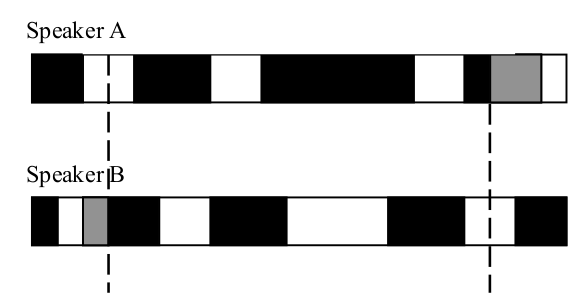
\includegraphics[width=10cm]{images/tama.png}
\caption{Gráfico de la separación del diálogo en ventanas}
\label{tama}
\end{figure}

Una vez que la conversación se ha partido en ventanas mediante el proceso descripto, se calculan los valores de la serie de tiempo para cada interlocutores de cada una de ellas. Ésto se hace mediante el siguiente cálculo:

\begin{equation}
    \mu = \sum\limits_{i=1}^N f_i d_i^\prime \label{eq:tama_mean}\\
\end{equation}

donde $i$ itera sobre las elocuciones dentro del \emph{frame}, $d_i^\prime$ es la duración relativa del segmento (respecto del tiempo total hablado) y $f_i$ es el valor de la \emph{feature} que estamos midiendo. $d_i^\prime$ se calcula con la fórmula

\begin{equation}
dr_i = \frac{d_i}{\sum\limits_{i=1}^N d_i}
\end{equation}

donde $d_i$ es la longitud en segundos de los segmentos del habla en el frame.

Como se ve en \ref{eq:tama_mean}, el valor que calculamos es una media ponderada del valor de la feature por la duración de las locuciones. Así, por ejemplo, al calcular una serie de tiempo sobre la intensidad, la contribución de interjecciones (\emph{ah!} por ejemplo), que suelen tener altos valores \emph{volumen}, estará disminuída por sus breves duraciones.

Una vez obtenidas, dado un feature acústico/prosódico y una conversación, dos series de tiempo mediante el cálculo ventana a ventana de \ref{eq:tama_mean}, necesitamos efectuar algún tipo de análisis sobre éstas para obtener una medida del \entrainment.

\nota{Mejorar el dibujo éste y agregarle una descripción}

\section{Series de Tiempo}
\label{sec:time_series}
\nota{Mandar ésto a un apéndice!}

\theoremstyle{definition}
\newtheorem{definicion}{Definición}

\subsection*{Definición Informal}
En términos informales, una serie de tiempo es un conjunto de datos recolectados secuencialmente en el tiempo. Este tipo de datos se dan en varios campos de estudio, como por ejemplo Economía, Ciencias de la Atmósfera, y otros.

Ejemplos de series de tiempo:

\begin{itemize}
    \item Volumen de lluvias en sucesivos días de un año
    \item Precio de acciones en diferentes meses
    \item Cantidad de habitantes de una ciudad año a año
\end{itemize}

\begin{figure}
\centering
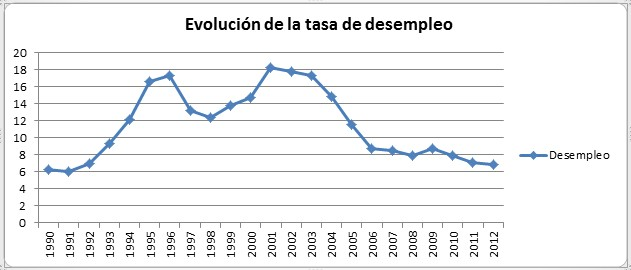
\includegraphics[width=15cm]{images/desocupacion.jpg}
\caption{Gráfico de serie de tiempo de la evolución del desempleo en Argentina \label{desocupacion}}
\end{figure}


\subsection*{¿Para qué queremos series de tiempo?}

Hay varios motivos por los cuales uno querría efectuar un análisis de una serie de tiempo.

\emph{1) Descripción} Usualmente, lo primero que se hace al obtener la serie de tiempo es graficarla y obtener las características más notorias de ésta. Por ejemplo, en \ref{desocupacion} puede notarse que hay una tendencia decreciente del $2003$ hasta el $2012$. En otras (como en el volumen de lluvias) podrá observarse cierta estacionalidad en la serie.

Si bien ésto no requiere técnicas avanzadas de análisis, es el primer paso fundamental para comprender una serie de tiempo.


\emph{2) Explicación} Cuando analizamos dos o más series de tiempo, podemos querer ver cómo se comportan en conjunto. Una variación en una serie de tiempo puede producir un cambio en otra. Por ejemplo, podemos intentar buscar como varían en conjunto la temperatura diaria con la cantidad de mL de lluvia caídos.

\emph{3) Predicción} Dada una serie de tiempo, podemos querer intentar predecir un valor futuro.

\emph{4) Control} Dado un proceso del que se mide cierto parámetro de calidad, podemos querer ajustar variables de entrada para mantenerla en ciertos valores.

En nuestro caso, nos es de interés 1 y 2.


\subsection{Procesos estocásticos}

\begin{definicion}
Una proceso estocástico es una colección de variables aleatorias $\{X_t \}_{t \in T}$ donde $T$ es un conjunto de puntos de tiempo. En nuestro caso, nos interesa $T = \mathbb{N}$, de manera que el proceso será de la forma $X_1, X_2, \ldots $
\end{definicion}

Podemos entender un proceso estocástico como un conjunto de variables ordenadas por el tiempo. Llamamos serie de tiempo a una observación de este proceso estocástico. Usualmente sólo tendremos esta instancia, a diferencia de otros problemas estadísticos donde tendremos muchas observaciones.


\subsection{Estacionariedad}

Un concepto importante en series de tiempo es el de estacionariedad. En lenguaje coloquial, una serie de tiempo estacionaria es aquella en la que no observamos cambios sistemáticos de ésta en el tiempo: si tomamos una parte de la serie, y observamos otro parte distinta de la serie, las propiedades de ésta se mantienen.

Ejemplos de series de tiempo estacionarias son las de ruido blanco, y ejemplos de no estacionarias aquellas que tienen una tendencia. (mejorar esto...)

\begin{definicion}
Un proceso estocástico $X_i, i \in \mathbb{N}$ se dice fuertemente estacionario si, para todo conjunto de índices $t_1, \ldots , t_n$ y para un desplazamiento $\tau \in \mathbb{N}$ tenemos que

\begin{displaymath}
    F_{X_{t_1}, X_{t_2}, \ldots , X_{t_n} } = F_{X_{t_1} + \tau, X_{t_2} + \tau, \ldots , X_{t_n} + \tau}
\end{displaymath}

Es decir, que la función de probabilidad se preserva por traslados.
\end{definicion}

Se derivan como propiedades que, para todo $X_t$ y cualquier desplazamiento $\tau$

\begin{align}
    E[X_t] &= E[X_{t + \tau}] \label{eq:1} \\
    Var[X_t] &= Var[X_{t + \tau}] \label{eq:2} \\
    Cov(X_s, X_t) &= Cov(X_{s+\tau}, X_{t + \tau}) \label{eq:3}
\end{align}

Las ecuaciones \ref{eq:1} y \ref{eq:2} nos dicen que tanto la media como la varianza son constantes (no dependen de $t$), y que la covarianza sólo depende de la diferencia $| s - t |$.


\begin{definicion}
    Un proceso se dice débilmente estacionario si cumple \ref{eq:1}, \ref{eq:2}, \ref{eq:3}
\end{definicion}

A partir de aquí, cuando hablemos de series estacionarias estaremos hablando de series débilmente estacionarias


\section{Análisis bivariado}
\label{sec:analisis_bivariado}

\newcommand{\squarederr}[1]{
    \sum\limits_{t=1}^n \varnorm{#1}^2
}

\newcommand{\crosscorr}[2]{
  \frac{\sum\limits_{t=|k|+1}^n \varnorm{#1} (#2_{t-k} - \mu_{#2})}{
    \sqrt{\squarederr{#1} \squarederr{#2}}
  } \\
}

\newcommand{\corrdenom}{\sqrt{\squarederr{A}\squarederr{B}}}

En \cite{KOU2008.2} se continúa el trabajo en series de tiempo, y se efectúan análisis tanto para cada serie por separado como para las dos en conjunto, lo cual se llama ``análisis bivariado'' en la terminología de series de tiempo. En este análisis pretendemos analizar ambas series como parte de un sistema y ver cómo se influyen y retroalimentan mutuamente.

Una posible medida del \entrainment se podría obtener midiendo cuánto influye una serie sobre otra, considerándolas a ambas como parte de un sistema donde ambas interactúan. Este \entrainment, entonces, sería direccional: queremos medir cuánto influye el interlocutor $A$ sobre el interlocutor $B$ y viceversa. Puede darse el caso en que ambos tengan fuerte interacción, en tal caso hablamos de \emph{feedback}.

Para medir cuánto se mimetizan las dos series, utilizaremos la función de correlación cruzada (f.c.c) \cite{CHATFIELD}, que mide cuánto se parecen la serie $X$ e $Y$ aplicando un desplazamiento $k$, lo cual nos arroja como resultado un valor entre $-1$ y $1$ (similar al coeficiente de correlación de la estadística clásica). Podemos aproximar la c.c.f. mediante la fórmula de la correlación cruzada muestral.

\begin{equation}
  \label{cross_correlation_definition}
  r_{AB}(k) =
  \left\{
    \begin{array}{ll}
      \frac{\sum\limits_{t=k+1}^n \varnorm{A} (B_{t-k} - \mu_{B})}{\corrdenom} \\ & \mbox{si } k \geq 0 \\
      \frac{\sum\limits_{t=-k+1}^n \varnorm{B} (A_{t+k} - \mu_{A})}{\corrdenom} \\  & \mbox{si } k < 0
    \end{array}
  \right.
\end{equation}

Podemos ver que, si $k \geq 0$, lo que hacemos es, a grandes rasgos, calcular la correlación de Pearson entre $A$ y $B$, pero tomando los $n-k$ últimos valores de $A$ y los $n-k$ primeros de $B$. Si $k < 0$, lo hacemos entre $A$ y $B$, pero desplazando en sentidos inversos. Viéndolo de otra forma, si $k \geq 0$, estamos midiendo cuánto influye $B$ sobre $A$ contemplando un desplazamiento de $k$ puntos; si $k \leq 0$ medimos la influencia de $A$ sobre $B$ a misma distancia. La utilización de estos desplazamientos está explicada en \cite{gravano2015backward}, donde se menciona que la influencia de los hablantes no es necesariamente inmediata sino que puede tener algunos segundos de demora para tomar lugar.


Para cada conversación, se estima entonces el correlograma cruzado, considerando desplazamientos tanto positivos como negativos. Hecho esto, en el estudio \cite{KOU2008.2} sólo analizan la significancia de los resultados de la correlación cruzada, enumerando aquellos lags en los cuales esto ocurrió. En la sección \ref{sec:method_entrainment} comentaremos cómo utilizamos la técnica descripta para la medición del entrainment direccional.

\begin{figure}
\centering
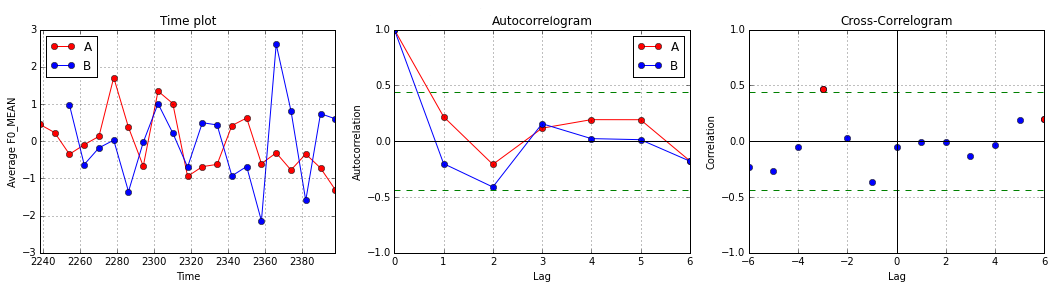
\includegraphics[width=15cm]{images/time_plot_with_cross_correlation.png}
\caption{Time-plot producido por TAMA, junto a su autocorrelación y correlación cruzada}
\end{figure}




\section{Materiales y Métodos}

\subsection{Corpus}
\begin{frame}
  \frametitle{Columbia Games Corpus}
  \framesubtitle{Descripción}
  \begin{columns}
    \column{0.35\textwidth}
      \begin{figure}
        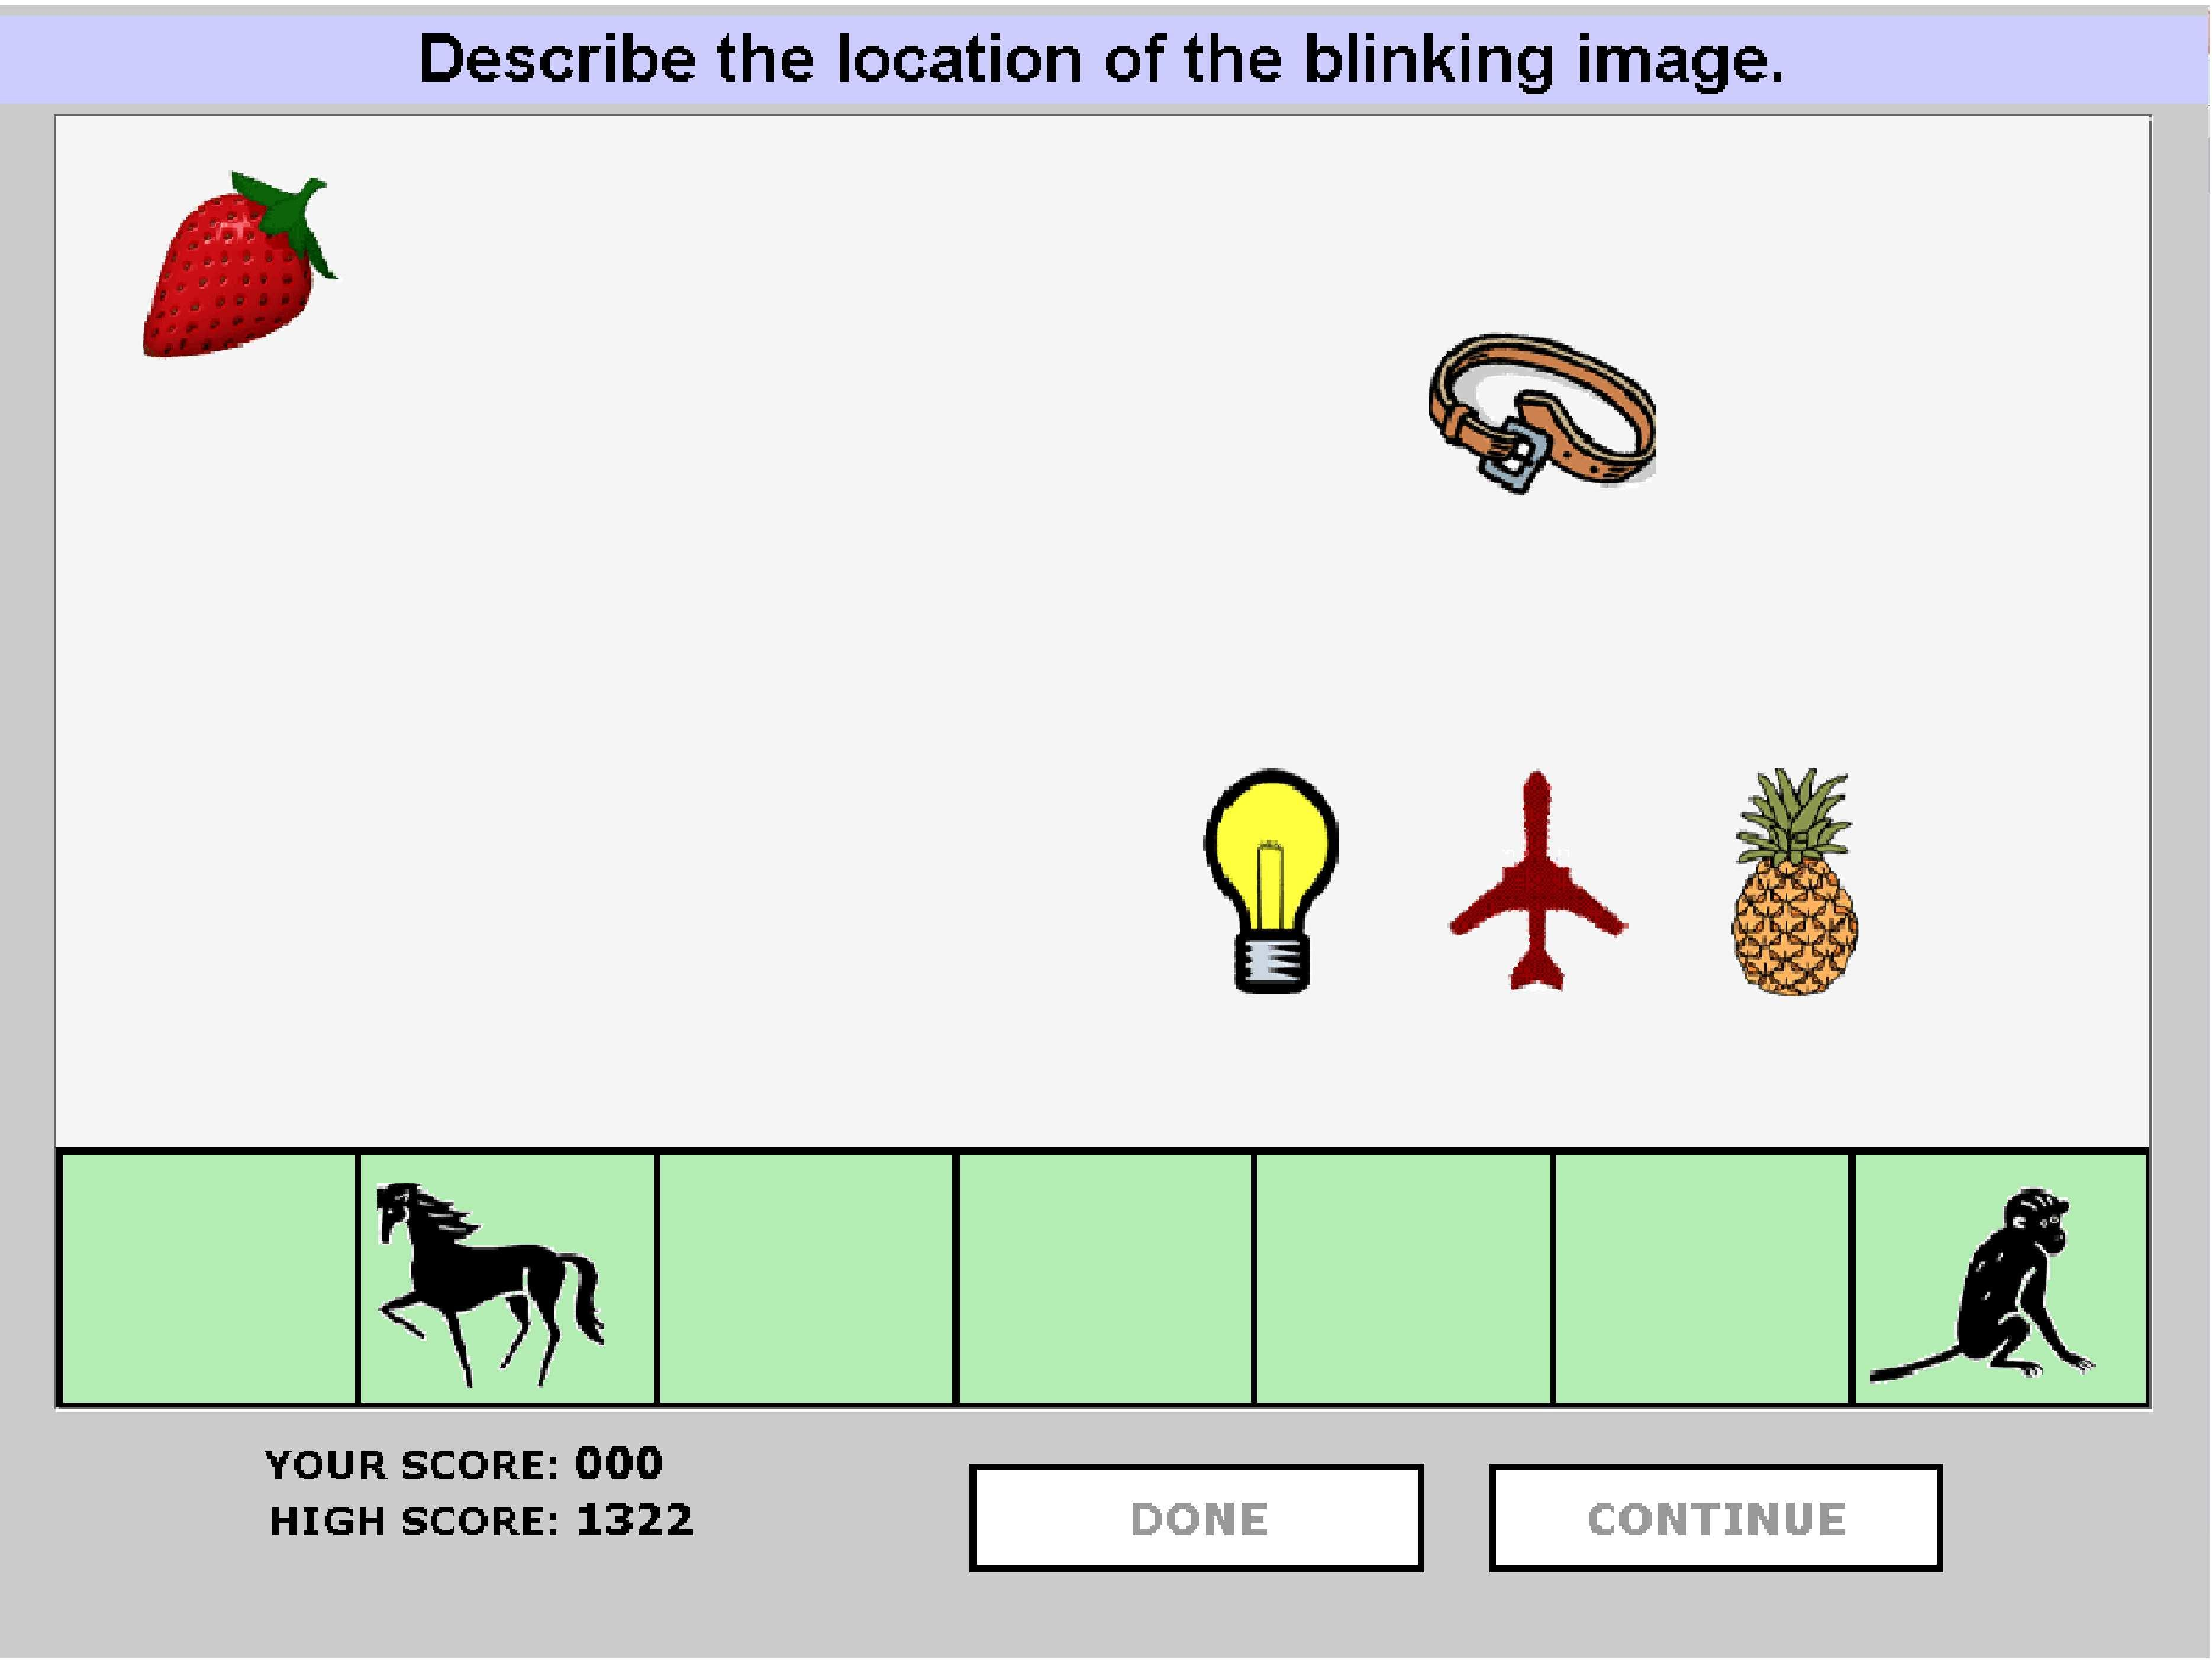
\includegraphics[width=\textwidth]{images/columbia_games_color.jpg}
      \end{figure}

    \column{0.65\textwidth}

    \begin{itemize}
      \item Corpus de conversaciones diádicas en Inglés Americano Estándar
      \item 12 sesiones con 14 tareas/juegos cada una.
      \item En cada sesión, se sentó a dos participantes en una cabina profesional de grabación, y una cortina opaca colgando entre ellos para evitar la comunicación visual.
      \item Los participantes contaron con computadoras a través de las cuales interactuaban mediante juegos.
    \end{itemize}
  \end{columns}

\end{frame}


\begin{frame}
  \frametitle{Columbia Games Corpus}
  \framesubtitle{Juegos de objeto}
  \begin{columns}
    \column{0.35\textwidth}
      \begin{figure}
        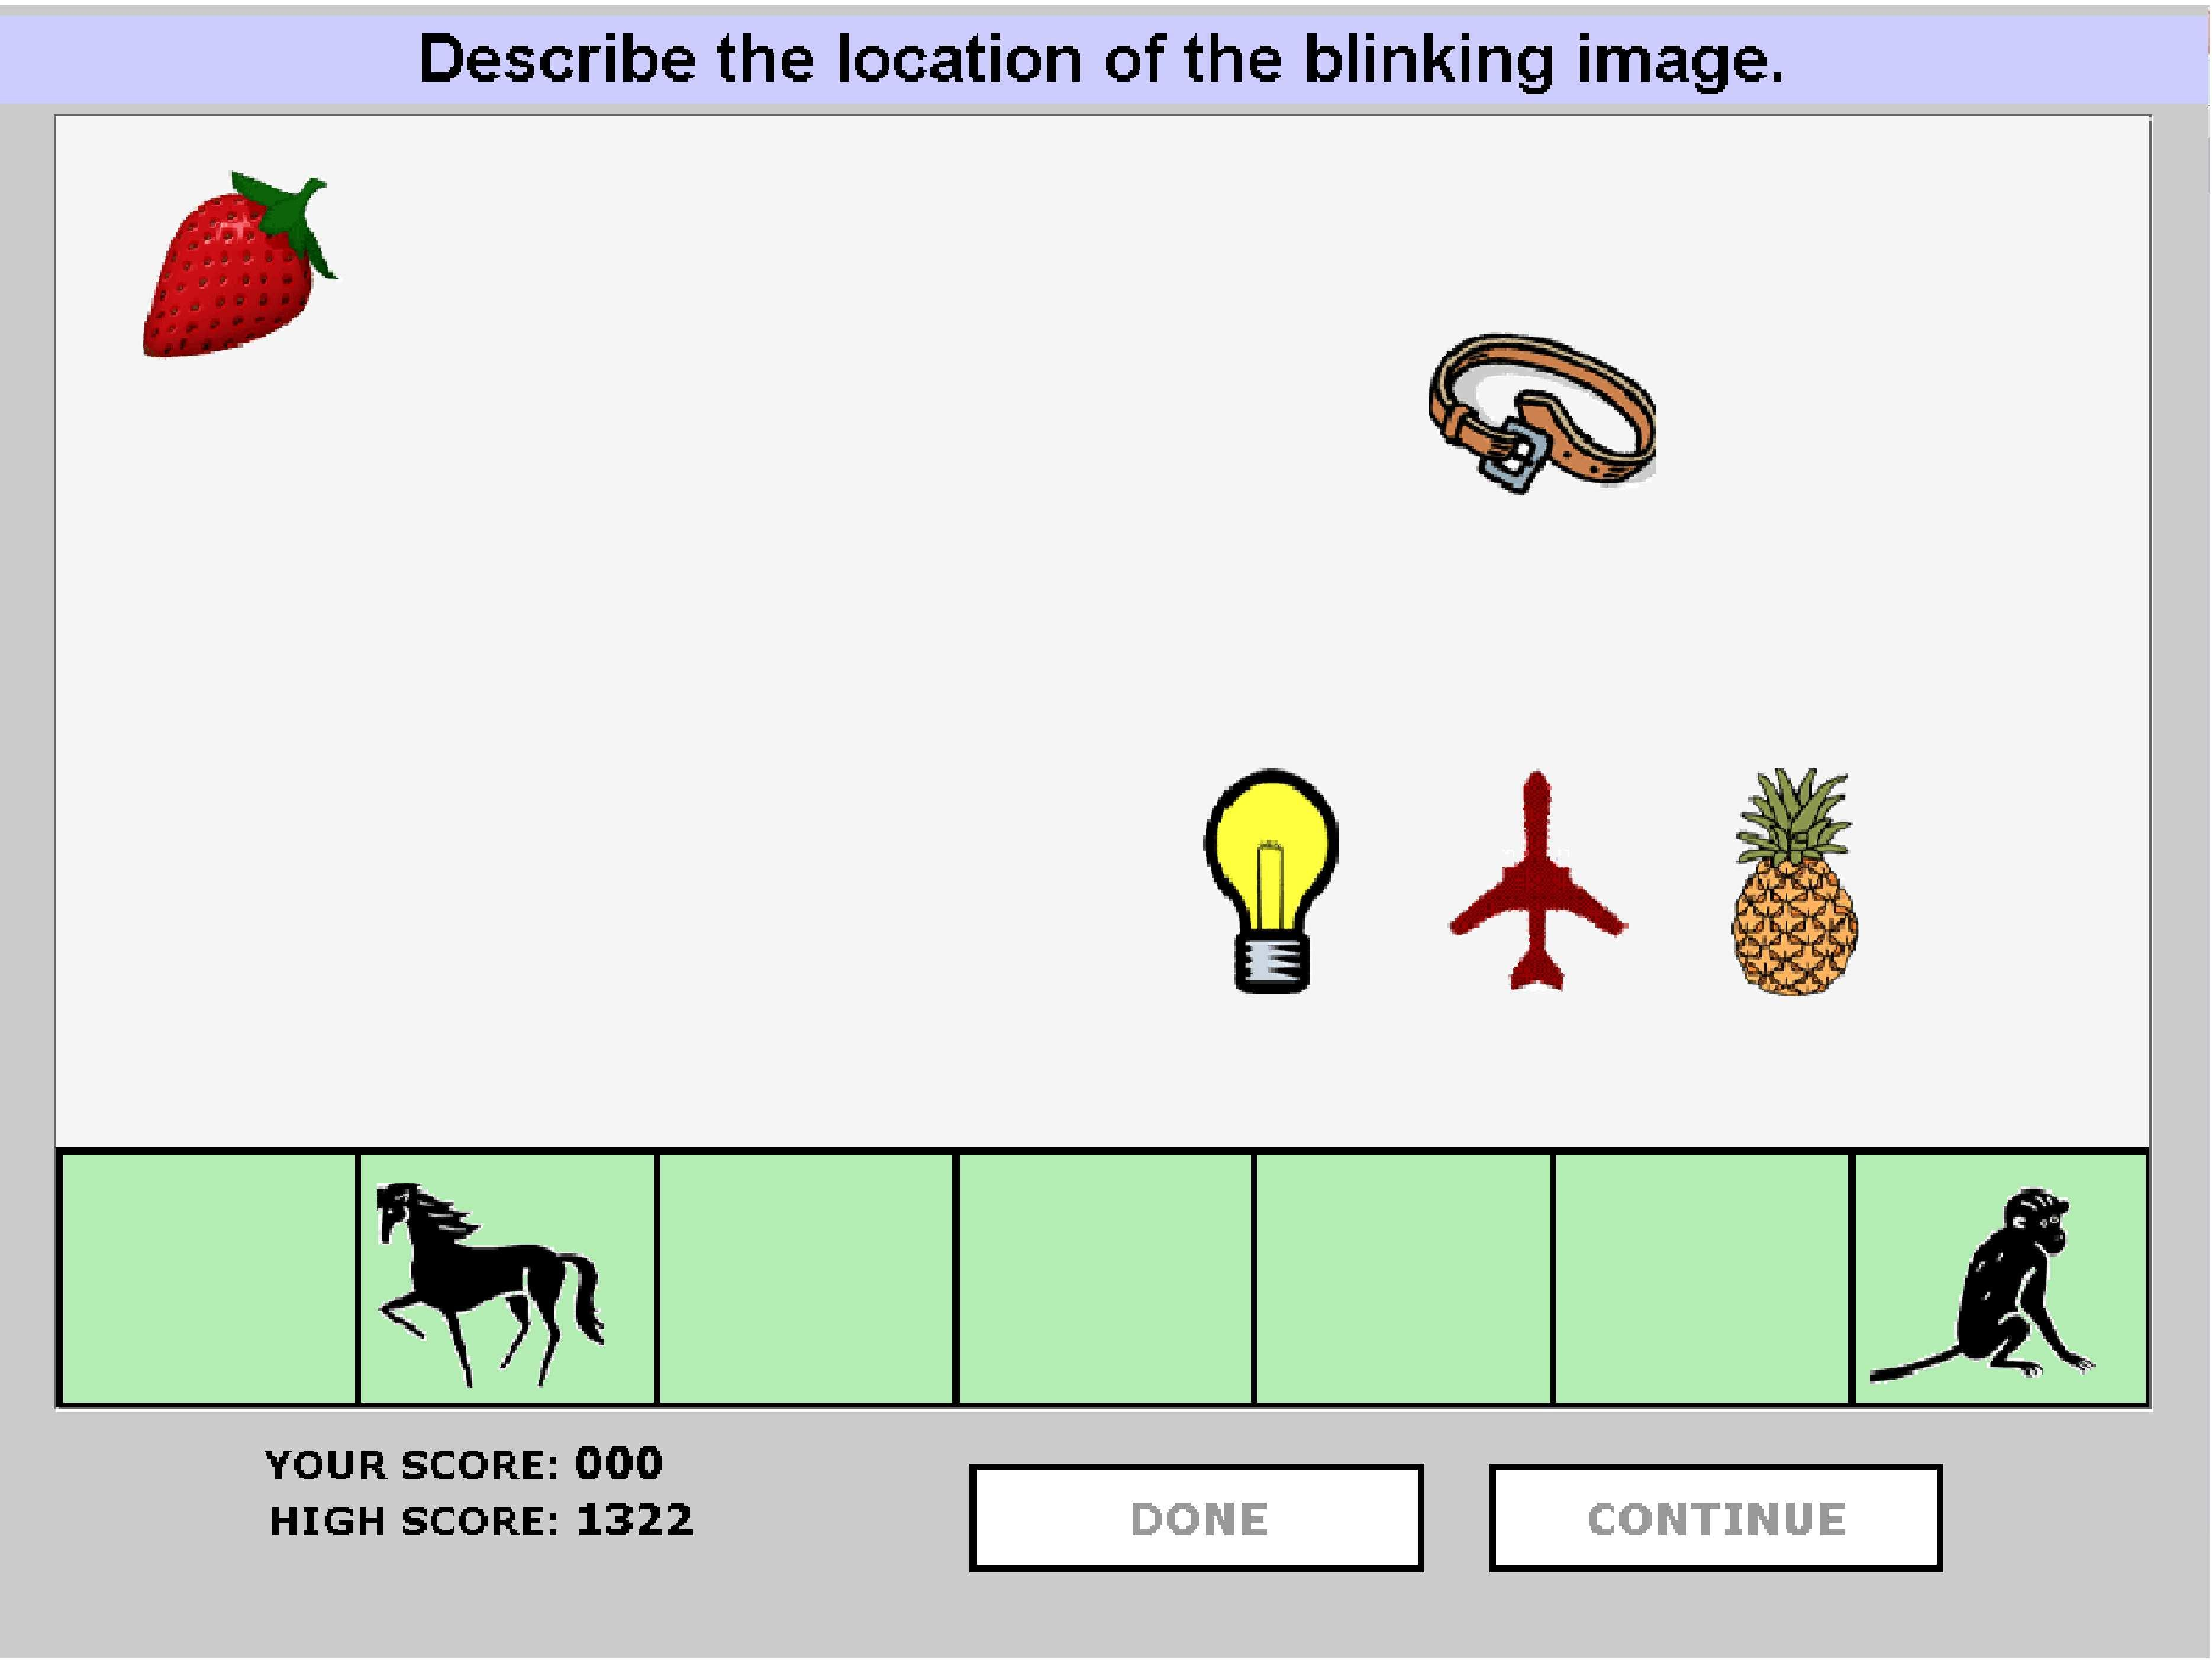
\includegraphics[width=\textwidth]{images/columbia_games_color.jpg}
      \end{figure}

    \column{0.65\textwidth}

    \begin{itemize}
      \item Dos roles: Descriptor y Seguidor
      \item En la pantalla, se ven entre 5 y 7 objetos en posiciones aleatorias
      \item El Descriptor ve uno más, titilante, del cual debe describir su posición
      \item El Seguidor debe mover la representación del objeto a la misma posición de la pantalla
      \item Finalmente, se puntúa de 1 a 100 el posicionamiento del objeto
    \end{itemize}
  \end{columns}
\end{frame}


\begin{frame}
  \frametitle{Columbia Games Corpus}
  \framesubtitle{Detalles y Anotaciones sociales}

\end{frame}




\end{document}
